%!TEX root = practicum2.tex
The performance of the perceptron trained with the Minover algorithm can be measured using the generalization error defined in \autoref{eq:method:generalization_error}. To explore the behaviour of the Minover algorithm discussed in section \ref{s:method} we have tested a perceptron trained with this algorithm on several $N$-dimensional datasets with $P = \alpha N$, for $N = 10$ and $\alpha = 0.25, 0.5, \dotsc, 5$. To ensure that the dataset was linearly separable we have determined its labels via \eqref{eq:method:teacher_label}, using the weight vector $\vec{w}^* = [1, \dotsc, 1]^T$.\\

\Cref{fig:exp:finalgeneralizationError} shows the final generalization error for different values of $\alpha$ as an average of 10 iterations with each $\alpha$. We consider a generalization error final when it has converged or when $t_{max}$ has been reached. 


\todo[inline]{Relatie tussen $\alpha$ en de generalisatie error.}
~\\

\begin{figure}
	\centering
	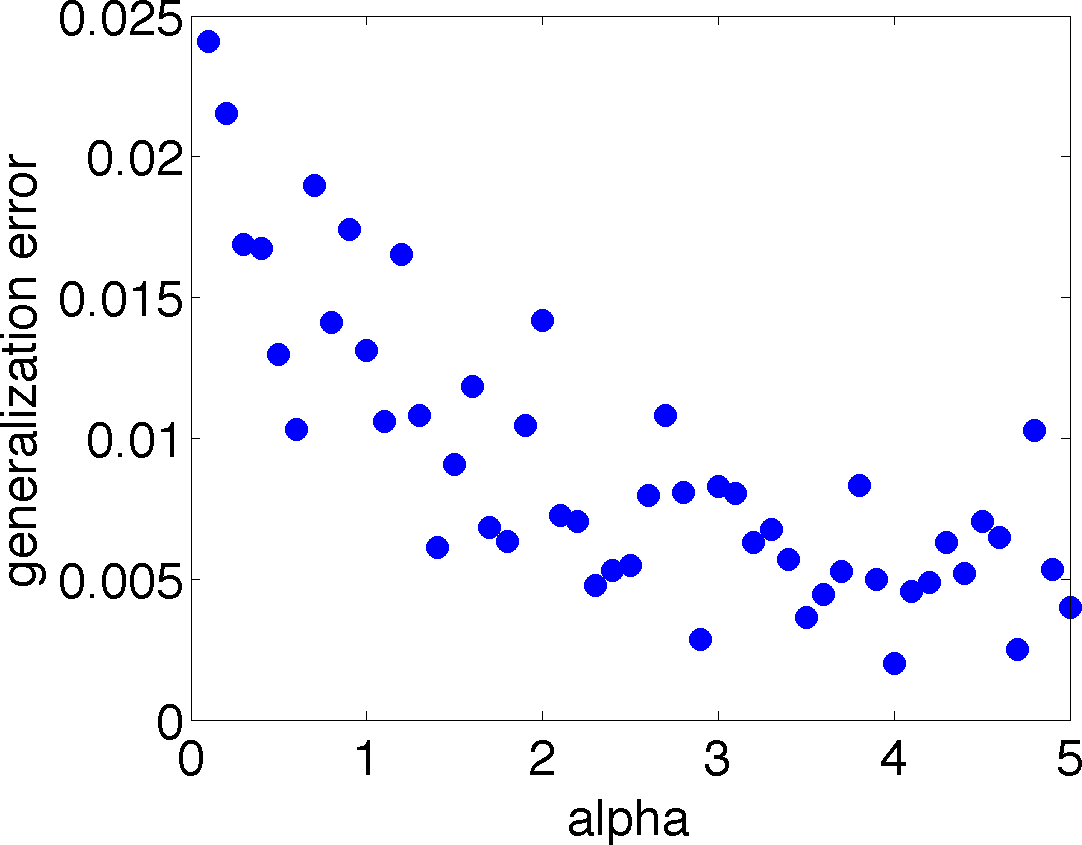
\includegraphics[width=0.9\columnwidth]{./img/finalgeneralizationerrors}
	\caption{Generalization error at the final step of training, for $\alpha = 0.25, 0.5, \dotsc, 5$, $\varepsilon = 0.0005$, $n_{max} = 500$ and $N = 10$.}
	\label{fig:exp:finalgeneralizationError}
\end{figure}

\Cref{fig:exp:learningcurve} shows the learning curves for different values of $\alpha$ for one dataset per $\alpha$. This figure clearly shows that for smaller values of $\alpha$ the algorithm needed less steps to converge. Furthermore for nearly all values of $\alpha$ the generalization decreased strongly before decreasingly oscillating around its final generalization error.

One possible explanation for these oscillations is that the optimal weights cannot be formulated as a linear combination of the support vectors. In this case the algorithm continues to add and subtract vectors from the weights, resulting in a constantly changing generalization error. Since our convergence criterion is the stabilization of the generalization error for $P$ steps, these oscillations prevent convergence. 

\todo[inline]{Waarom hebben kleinere datasets minder lang nogdig om te convergeren?}

\begin{figure}
	\centering
	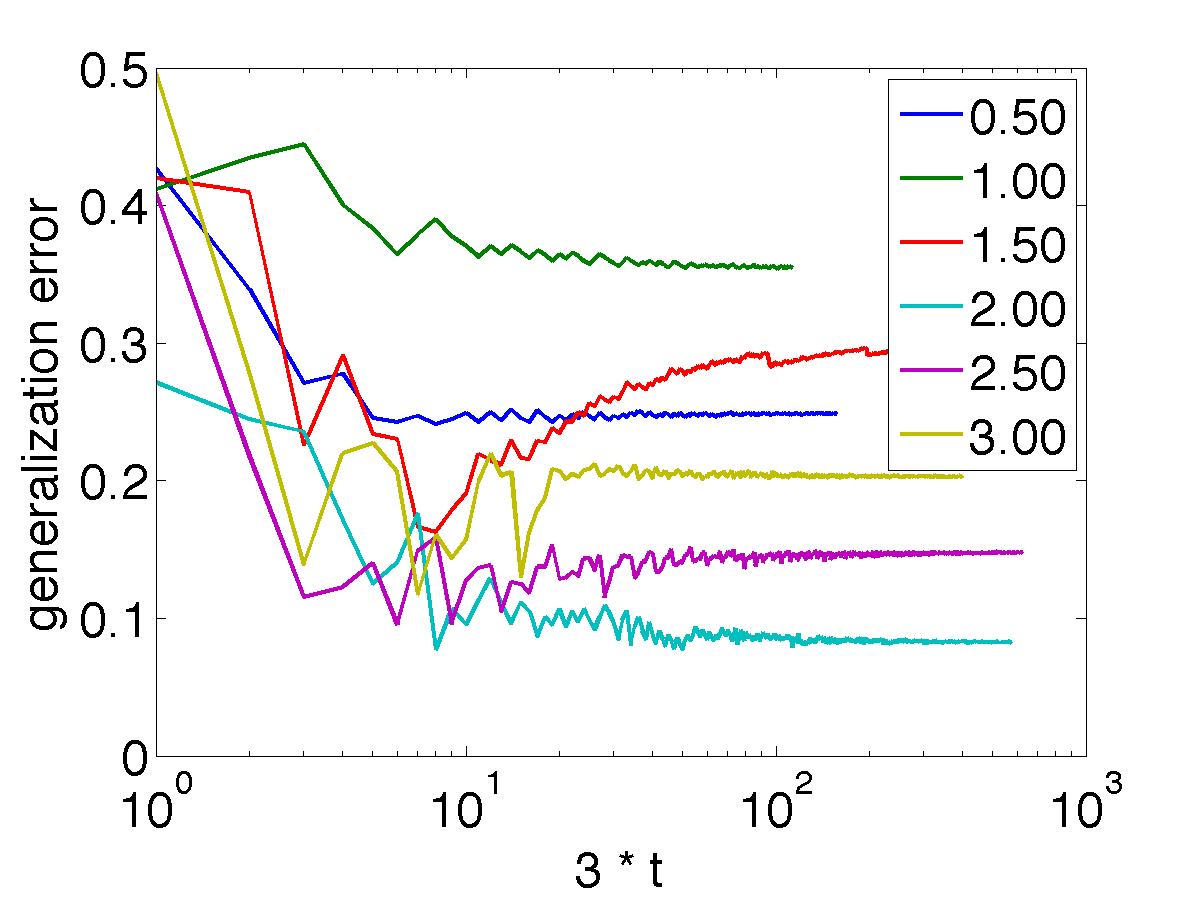
\includegraphics[width=0.9\columnwidth]{./img/N5NMAX500error3}
	\caption{Learning curve for different $\alpha$ for $N = 5$, and $\varepsilon = 0.0005$ and $n_{max} = 500$.}
	\label{fig:exp:learningcurve}
\end{figure}